% Created by tikzDevice version 0.12.6 on 2025-08-19 18:36:07
% !TEX encoding = UTF-8 Unicode
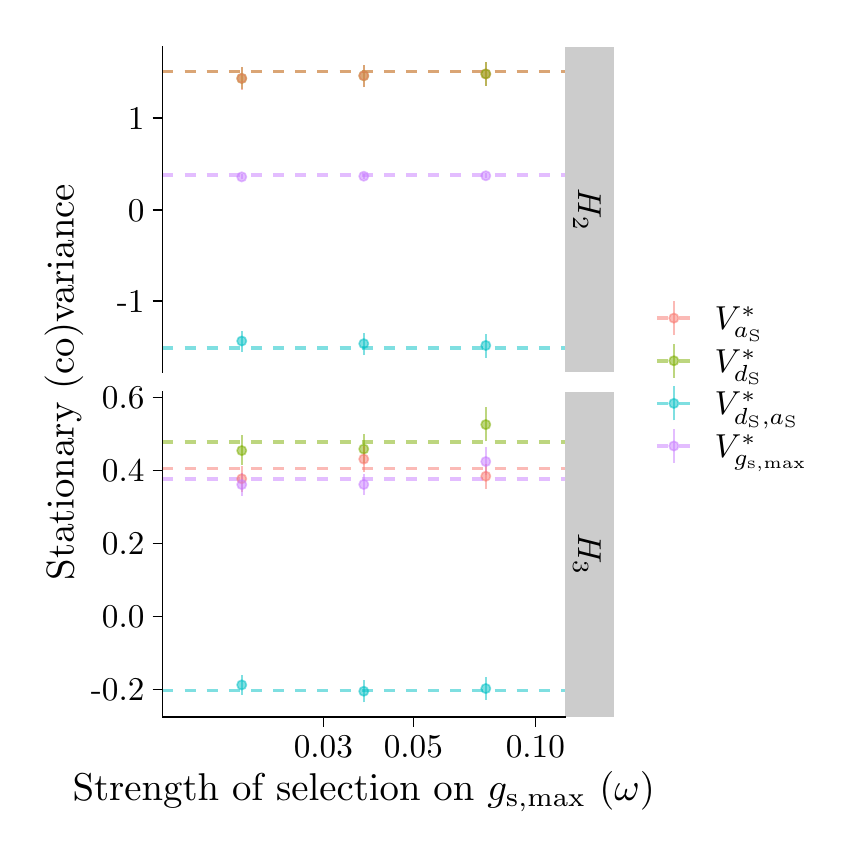
\begin{tikzpicture}[x=1pt,y=1pt]
\definecolor{fillColor}{RGB}{255,255,255}
\path[use as bounding box,fill=fillColor,fill opacity=0.00] (0,0) rectangle (289.08,289.08);
\begin{scope}
\path[clip] ( 48.69,164.52) rectangle (194.20,282.08);
\definecolor{drawColor}{RGB}{124,174,0}

\path[draw=drawColor,draw opacity=0.50,line width= 1.3pt,dash pattern=on 4pt off 4pt ,line join=round] ( 48.69,273.24) -- (194.20,273.24);
\definecolor{drawColor}{RGB}{248,118,109}

\path[draw=drawColor,draw opacity=0.50,line width= 1.3pt,dash pattern=on 4pt off 4pt ,line join=round] ( 48.69,273.24) -- (194.20,273.24);
\definecolor{drawColor}{RGB}{0,191,196}

\path[draw=drawColor,draw opacity=0.50,line width= 1.3pt,dash pattern=on 4pt off 4pt ,line join=round] ( 48.69,173.36) -- (194.20,173.36);
\definecolor{drawColor}{RGB}{199,124,255}

\path[draw=drawColor,draw opacity=0.50,line width= 1.3pt,dash pattern=on 4pt off 4pt ,line join=round] ( 48.69,235.79) -- (194.20,235.79);
\definecolor{drawColor}{RGB}{248,118,109}

\path[draw=drawColor,draw opacity=0.50,line width= 0.7pt,line join=round] (165.54,268.03) -- (165.54,276.74);
\definecolor{drawColor}{RGB}{124,174,0}

\path[draw=drawColor,draw opacity=0.50,line width= 0.7pt,line join=round] (165.54,268.02) -- (165.54,276.69);
\definecolor{drawColor}{RGB}{0,191,196}

\path[draw=drawColor,draw opacity=0.50,line width= 0.7pt,line join=round] (165.54,169.86) -- (165.54,178.41);
\definecolor{drawColor}{RGB}{124,174,0}

\path[draw=drawColor,draw opacity=0.50,line width= 0.7pt,line join=round] ( 77.35,266.93) -- ( 77.35,275.03);
\definecolor{drawColor}{RGB}{248,118,109}

\path[draw=drawColor,draw opacity=0.50,line width= 0.7pt,line join=round] ( 77.35,266.70) -- ( 77.35,274.78);
\definecolor{drawColor}{RGB}{124,174,0}

\path[draw=drawColor,draw opacity=0.50,line width= 0.7pt,line join=round] (121.45,267.76) -- (121.45,275.69);
\definecolor{drawColor}{RGB}{248,118,109}

\path[draw=drawColor,draw opacity=0.50,line width= 0.7pt,line join=round] (121.45,267.50) -- (121.45,275.42);
\definecolor{drawColor}{RGB}{0,191,196}

\path[draw=drawColor,draw opacity=0.50,line width= 0.7pt,line join=round] (121.45,170.78) -- (121.45,178.68);

\path[draw=drawColor,draw opacity=0.50,line width= 0.7pt,line join=round] ( 77.35,171.98) -- ( 77.35,179.55);
\definecolor{drawColor}{RGB}{199,124,255}

\path[draw=drawColor,draw opacity=0.50,line width= 0.7pt,line join=round] (165.54,234.59) -- (165.54,236.67);

\path[draw=drawColor,draw opacity=0.50,line width= 0.7pt,line join=round] (121.45,234.40) -- (121.45,236.38);

\path[draw=drawColor,draw opacity=0.50,line width= 0.7pt,line join=round] ( 77.35,234.27) -- ( 77.35,236.12);
\definecolor{drawColor}{RGB}{248,118,109}
\definecolor{fillColor}{RGB}{248,118,109}

\path[draw=drawColor,draw opacity=0.50,line width= 0.6pt,line join=round,line cap=round,fill=fillColor,fill opacity=0.50] (165.54,272.35) circle (  1.69);
\definecolor{drawColor}{RGB}{124,174,0}
\definecolor{fillColor}{RGB}{124,174,0}

\path[draw=drawColor,draw opacity=0.50,line width= 0.6pt,line join=round,line cap=round,fill=fillColor,fill opacity=0.50] (165.54,272.36) circle (  1.69);
\definecolor{drawColor}{RGB}{0,191,196}
\definecolor{fillColor}{RGB}{0,191,196}

\path[draw=drawColor,draw opacity=0.50,line width= 0.6pt,line join=round,line cap=round,fill=fillColor,fill opacity=0.50] (165.54,174.25) circle (  1.69);
\definecolor{drawColor}{RGB}{124,174,0}
\definecolor{fillColor}{RGB}{124,174,0}

\path[draw=drawColor,draw opacity=0.50,line width= 0.6pt,line join=round,line cap=round,fill=fillColor,fill opacity=0.50] ( 77.35,270.74) circle (  1.69);
\definecolor{drawColor}{RGB}{248,118,109}
\definecolor{fillColor}{RGB}{248,118,109}

\path[draw=drawColor,draw opacity=0.50,line width= 0.6pt,line join=round,line cap=round,fill=fillColor,fill opacity=0.50] ( 77.35,270.76) circle (  1.69);
\definecolor{drawColor}{RGB}{124,174,0}
\definecolor{fillColor}{RGB}{124,174,0}

\path[draw=drawColor,draw opacity=0.50,line width= 0.6pt,line join=round,line cap=round,fill=fillColor,fill opacity=0.50] (121.45,271.70) circle (  1.69);
\definecolor{drawColor}{RGB}{248,118,109}
\definecolor{fillColor}{RGB}{248,118,109}

\path[draw=drawColor,draw opacity=0.50,line width= 0.6pt,line join=round,line cap=round,fill=fillColor,fill opacity=0.50] (121.45,271.72) circle (  1.69);
\definecolor{drawColor}{RGB}{0,191,196}
\definecolor{fillColor}{RGB}{0,191,196}

\path[draw=drawColor,draw opacity=0.50,line width= 0.6pt,line join=round,line cap=round,fill=fillColor,fill opacity=0.50] (121.45,174.89) circle (  1.69);

\path[draw=drawColor,draw opacity=0.50,line width= 0.6pt,line join=round,line cap=round,fill=fillColor,fill opacity=0.50] ( 77.35,175.85) circle (  1.69);
\definecolor{drawColor}{RGB}{199,124,255}
\definecolor{fillColor}{RGB}{199,124,255}

\path[draw=drawColor,draw opacity=0.50,line width= 0.6pt,line join=round,line cap=round,fill=fillColor,fill opacity=0.50] (165.54,235.57) circle (  1.69);

\path[draw=drawColor,draw opacity=0.50,line width= 0.6pt,line join=round,line cap=round,fill=fillColor,fill opacity=0.50] (121.45,235.40) circle (  1.69);

\path[draw=drawColor,draw opacity=0.50,line width= 0.6pt,line join=round,line cap=round,fill=fillColor,fill opacity=0.50] ( 77.35,235.16) circle (  1.69);
\end{scope}
\begin{scope}
\path[clip] ( 48.69, 39.96) rectangle (194.20,157.52);
\definecolor{drawColor}{RGB}{124,174,0}

\path[draw=drawColor,draw opacity=0.50,line width= 1.3pt,dash pattern=on 4pt off 4pt ,line join=round] ( 48.69,139.44) -- (194.20,139.44);
\definecolor{drawColor}{RGB}{248,118,109}

\path[draw=drawColor,draw opacity=0.50,line width= 1.3pt,dash pattern=on 4pt off 4pt ,line join=round] ( 48.69,129.72) -- (194.20,129.72);
\definecolor{drawColor}{RGB}{0,191,196}

\path[draw=drawColor,draw opacity=0.50,line width= 1.3pt,dash pattern=on 4pt off 4pt ,line join=round] ( 48.69, 49.61) -- (194.20, 49.61);
\definecolor{drawColor}{RGB}{199,124,255}

\path[draw=drawColor,draw opacity=0.50,line width= 1.3pt,dash pattern=on 4pt off 4pt ,line join=round] ( 48.69,126.09) -- (194.20,126.09);
\definecolor{drawColor}{RGB}{124,174,0}

\path[draw=drawColor,draw opacity=0.50,line width= 0.7pt,line join=round] (165.54,139.61) -- (165.54,152.18);

\path[draw=drawColor,draw opacity=0.50,line width= 0.7pt,line join=round] ( 77.35,131.15) -- ( 77.35,141.79);

\path[draw=drawColor,draw opacity=0.50,line width= 0.7pt,line join=round] (121.45,131.95) -- (121.45,142.32);
\definecolor{drawColor}{RGB}{199,124,255}

\path[draw=drawColor,draw opacity=0.50,line width= 0.7pt,line join=round] (165.54,127.30) -- (165.54,137.52);
\definecolor{drawColor}{RGB}{248,118,109}

\path[draw=drawColor,draw opacity=0.50,line width= 0.7pt,line join=round] ( 77.35,121.32) -- ( 77.35,130.64);

\path[draw=drawColor,draw opacity=0.50,line width= 0.7pt,line join=round] (165.54,122.33) -- (165.54,131.49);

\path[draw=drawColor,draw opacity=0.50,line width= 0.7pt,line join=round] (121.45,128.67) -- (121.45,137.74);
\definecolor{drawColor}{RGB}{199,124,255}

\path[draw=drawColor,draw opacity=0.50,line width= 0.7pt,line join=round] ( 77.35,119.77) -- ( 77.35,128.03);
\definecolor{drawColor}{RGB}{0,191,196}

\path[draw=drawColor,draw opacity=0.50,line width= 0.7pt,line join=round] (165.54, 46.19) -- (165.54, 54.27);

\path[draw=drawColor,draw opacity=0.50,line width= 0.7pt,line join=round] (121.45, 45.30) -- (121.45, 53.36);
\definecolor{drawColor}{RGB}{199,124,255}

\path[draw=drawColor,draw opacity=0.50,line width= 0.7pt,line join=round] (121.45,120.12) -- (121.45,127.87);
\definecolor{drawColor}{RGB}{0,191,196}

\path[draw=drawColor,draw opacity=0.50,line width= 0.7pt,line join=round] ( 77.35, 47.97) -- ( 77.35, 55.30);
\definecolor{drawColor}{RGB}{124,174,0}
\definecolor{fillColor}{RGB}{124,174,0}

\path[draw=drawColor,draw opacity=0.50,line width= 0.6pt,line join=round,line cap=round,fill=fillColor,fill opacity=0.50] (165.54,145.66) circle (  1.69);

\path[draw=drawColor,draw opacity=0.50,line width= 0.6pt,line join=round,line cap=round,fill=fillColor,fill opacity=0.50] ( 77.35,136.26) circle (  1.69);

\path[draw=drawColor,draw opacity=0.50,line width= 0.6pt,line join=round,line cap=round,fill=fillColor,fill opacity=0.50] (121.45,136.82) circle (  1.69);
\definecolor{drawColor}{RGB}{199,124,255}
\definecolor{fillColor}{RGB}{199,124,255}

\path[draw=drawColor,draw opacity=0.50,line width= 0.6pt,line join=round,line cap=round,fill=fillColor,fill opacity=0.50] (165.54,132.29) circle (  1.69);
\definecolor{drawColor}{RGB}{248,118,109}
\definecolor{fillColor}{RGB}{248,118,109}

\path[draw=drawColor,draw opacity=0.50,line width= 0.6pt,line join=round,line cap=round,fill=fillColor,fill opacity=0.50] ( 77.35,126.08) circle (  1.69);

\path[draw=drawColor,draw opacity=0.50,line width= 0.6pt,line join=round,line cap=round,fill=fillColor,fill opacity=0.50] (165.54,126.99) circle (  1.69);

\path[draw=drawColor,draw opacity=0.50,line width= 0.6pt,line join=round,line cap=round,fill=fillColor,fill opacity=0.50] (121.45,133.19) circle (  1.69);
\definecolor{drawColor}{RGB}{199,124,255}
\definecolor{fillColor}{RGB}{199,124,255}

\path[draw=drawColor,draw opacity=0.50,line width= 0.6pt,line join=round,line cap=round,fill=fillColor,fill opacity=0.50] ( 77.35,123.98) circle (  1.69);
\definecolor{drawColor}{RGB}{0,191,196}
\definecolor{fillColor}{RGB}{0,191,196}

\path[draw=drawColor,draw opacity=0.50,line width= 0.6pt,line join=round,line cap=round,fill=fillColor,fill opacity=0.50] (165.54, 50.28) circle (  1.69);

\path[draw=drawColor,draw opacity=0.50,line width= 0.6pt,line join=round,line cap=round,fill=fillColor,fill opacity=0.50] (121.45, 49.30) circle (  1.69);
\definecolor{drawColor}{RGB}{199,124,255}
\definecolor{fillColor}{RGB}{199,124,255}

\path[draw=drawColor,draw opacity=0.50,line width= 0.6pt,line join=round,line cap=round,fill=fillColor,fill opacity=0.50] (121.45,124.02) circle (  1.69);
\definecolor{drawColor}{RGB}{0,191,196}
\definecolor{fillColor}{RGB}{0,191,196}

\path[draw=drawColor,draw opacity=0.50,line width= 0.6pt,line join=round,line cap=round,fill=fillColor,fill opacity=0.50] ( 77.35, 51.59) circle (  1.69);
\end{scope}
\begin{scope}
\path[clip] (194.20,164.52) rectangle (211.80,282.08);
\definecolor{fillColor}{gray}{0.80}

\path[fill=fillColor] (194.20,164.52) rectangle (211.80,282.08);
\definecolor{drawColor}{RGB}{0,0,0}

\node[text=drawColor,rotate=-90.00,anchor=base,inner sep=0pt, outer sep=0pt, scale=  1.20] at (198.87,223.30) {$H_2$};
\end{scope}
\begin{scope}
\path[clip] (194.20, 39.96) rectangle (211.80,157.52);
\definecolor{fillColor}{gray}{0.80}

\path[fill=fillColor] (194.20, 39.96) rectangle (211.80,157.52);
\definecolor{drawColor}{RGB}{0,0,0}

\node[text=drawColor,rotate=-90.00,anchor=base,inner sep=0pt, outer sep=0pt, scale=  1.20] at (198.87, 98.74) {$H_3$};
\end{scope}
\begin{scope}
\path[clip] (  0.00,  0.00) rectangle (289.08,289.08);
\definecolor{drawColor}{RGB}{0,0,0}

\path[draw=drawColor,line width= 0.6pt,line join=round,line cap=rect] ( 48.69, 39.96) --
	(194.20, 39.96);
\end{scope}
\begin{scope}
\path[clip] (  0.00,  0.00) rectangle (289.08,289.08);
\definecolor{drawColor}{RGB}{0,0,0}

\path[draw=drawColor,line width= 0.6pt,line join=round] (106.86, 36.46) --
	(106.86, 39.96);

\path[draw=drawColor,line width= 0.6pt,line join=round] (139.36, 36.46) --
	(139.36, 39.96);

\path[draw=drawColor,line width= 0.6pt,line join=round] (183.45, 36.46) --
	(183.45, 39.96);
\end{scope}
\begin{scope}
\path[clip] (  0.00,  0.00) rectangle (289.08,289.08);
\definecolor{drawColor}{RGB}{0,0,0}

\node[text=drawColor,anchor=base,inner sep=0pt, outer sep=0pt, scale=  1.20] at (106.86, 25.20) {0.03};

\node[text=drawColor,anchor=base,inner sep=0pt, outer sep=0pt, scale=  1.20] at (139.36, 25.20) {0.05};

\node[text=drawColor,anchor=base,inner sep=0pt, outer sep=0pt, scale=  1.20] at (183.45, 25.20) {0.10};
\end{scope}
\begin{scope}
\path[clip] (  0.00,  0.00) rectangle (289.08,289.08);
\definecolor{drawColor}{RGB}{0,0,0}

\path[draw=drawColor,line width= 0.6pt,line join=round,line cap=rect] ( 48.69,164.52) --
	( 48.69,282.08);
\end{scope}
\begin{scope}
\path[clip] (  0.00,  0.00) rectangle (289.08,289.08);
\definecolor{drawColor}{RGB}{0,0,0}

\node[text=drawColor,anchor=base east,inner sep=0pt, outer sep=0pt, scale=  1.20] at ( 42.19,186.08) {-1};

\node[text=drawColor,anchor=base east,inner sep=0pt, outer sep=0pt, scale=  1.20] at ( 42.19,219.17) {0};

\node[text=drawColor,anchor=base east,inner sep=0pt, outer sep=0pt, scale=  1.20] at ( 42.19,252.26) {1};
\end{scope}
\begin{scope}
\path[clip] (  0.00,  0.00) rectangle (289.08,289.08);
\definecolor{drawColor}{RGB}{0,0,0}

\path[draw=drawColor,line width= 0.6pt,line join=round] ( 45.19,190.21) --
	( 48.69,190.21);

\path[draw=drawColor,line width= 0.6pt,line join=round] ( 45.19,223.30) --
	( 48.69,223.30);

\path[draw=drawColor,line width= 0.6pt,line join=round] ( 45.19,256.39) --
	( 48.69,256.39);
\end{scope}
\begin{scope}
\path[clip] (  0.00,  0.00) rectangle (289.08,289.08);
\definecolor{drawColor}{RGB}{0,0,0}

\path[draw=drawColor,line width= 0.6pt,line join=round,line cap=rect] ( 48.69, 39.96) --
	( 48.69,157.52);
\end{scope}
\begin{scope}
\path[clip] (  0.00,  0.00) rectangle (289.08,289.08);
\definecolor{drawColor}{RGB}{0,0,0}

\node[text=drawColor,anchor=base east,inner sep=0pt, outer sep=0pt, scale=  1.20] at ( 42.19, 45.79) {-0.2};

\node[text=drawColor,anchor=base east,inner sep=0pt, outer sep=0pt, scale=  1.20] at ( 42.19, 72.18) {0.0};

\node[text=drawColor,anchor=base east,inner sep=0pt, outer sep=0pt, scale=  1.20] at ( 42.19, 98.57) {0.2};

\node[text=drawColor,anchor=base east,inner sep=0pt, outer sep=0pt, scale=  1.20] at ( 42.19,124.95) {0.4};

\node[text=drawColor,anchor=base east,inner sep=0pt, outer sep=0pt, scale=  1.20] at ( 42.19,151.34) {0.6};
\end{scope}
\begin{scope}
\path[clip] (  0.00,  0.00) rectangle (289.08,289.08);
\definecolor{drawColor}{RGB}{0,0,0}

\path[draw=drawColor,line width= 0.6pt,line join=round] ( 45.19, 49.93) --
	( 48.69, 49.93);

\path[draw=drawColor,line width= 0.6pt,line join=round] ( 45.19, 76.31) --
	( 48.69, 76.31);

\path[draw=drawColor,line width= 0.6pt,line join=round] ( 45.19,102.70) --
	( 48.69,102.70);

\path[draw=drawColor,line width= 0.6pt,line join=round] ( 45.19,129.08) --
	( 48.69,129.08);

\path[draw=drawColor,line width= 0.6pt,line join=round] ( 45.19,155.47) --
	( 48.69,155.47);
\end{scope}
\begin{scope}
\path[clip] (  0.00,  0.00) rectangle (289.08,289.08);
\definecolor{drawColor}{RGB}{0,0,0}

\node[text=drawColor,anchor=base,inner sep=0pt, outer sep=0pt, scale=  1.40] at (121.45,  9.72) {Strength of selection on $g_\mathrm{s,max}$ ($\omega$)};
\end{scope}
\begin{scope}
\path[clip] (  0.00,  0.00) rectangle (289.08,289.08);
\definecolor{drawColor}{RGB}{0,0,0}

\node[text=drawColor,rotate= 90.00,anchor=base,inner sep=0pt, outer sep=0pt, scale=  1.40] at ( 16.64,161.02) {Stationary (co)variance};
\end{scope}
\begin{scope}
\path[clip] (  0.00,  0.00) rectangle (289.08,289.08);
\definecolor{drawColor}{RGB}{248,118,109}

\path[draw=drawColor,draw opacity=0.50,line width= 1.3pt,dash pattern=on 4pt off 4pt ,line join=round] (227.34,184.12) -- (239.66,184.12);
\end{scope}
\begin{scope}
\path[clip] (  0.00,  0.00) rectangle (289.08,289.08);
\definecolor{drawColor}{RGB}{248,118,109}

\path[draw=drawColor,draw opacity=0.50,line width= 0.7pt,line join=round] (233.50,177.96) -- (233.50,190.28);
\definecolor{fillColor}{RGB}{248,118,109}

\path[draw=drawColor,draw opacity=0.50,line width= 0.6pt,line join=round,line cap=round,fill=fillColor,fill opacity=0.50] (233.50,184.12) circle (  1.69);
\end{scope}
\begin{scope}
\path[clip] (  0.00,  0.00) rectangle (289.08,289.08);
\definecolor{drawColor}{RGB}{124,174,0}

\path[draw=drawColor,draw opacity=0.50,line width= 1.3pt,dash pattern=on 4pt off 4pt ,line join=round] (227.34,168.72) -- (239.66,168.72);
\end{scope}
\begin{scope}
\path[clip] (  0.00,  0.00) rectangle (289.08,289.08);
\definecolor{drawColor}{RGB}{124,174,0}

\path[draw=drawColor,draw opacity=0.50,line width= 0.7pt,line join=round] (233.50,162.56) -- (233.50,174.88);
\definecolor{fillColor}{RGB}{124,174,0}

\path[draw=drawColor,draw opacity=0.50,line width= 0.6pt,line join=round,line cap=round,fill=fillColor,fill opacity=0.50] (233.50,168.72) circle (  1.69);
\end{scope}
\begin{scope}
\path[clip] (  0.00,  0.00) rectangle (289.08,289.08);
\definecolor{drawColor}{RGB}{0,191,196}

\path[draw=drawColor,draw opacity=0.50,line width= 1.3pt,dash pattern=on 4pt off 4pt ,line join=round] (227.34,153.32) -- (239.66,153.32);
\end{scope}
\begin{scope}
\path[clip] (  0.00,  0.00) rectangle (289.08,289.08);
\definecolor{drawColor}{RGB}{0,191,196}

\path[draw=drawColor,draw opacity=0.50,line width= 0.7pt,line join=round] (233.50,147.16) -- (233.50,159.48);
\definecolor{fillColor}{RGB}{0,191,196}

\path[draw=drawColor,draw opacity=0.50,line width= 0.6pt,line join=round,line cap=round,fill=fillColor,fill opacity=0.50] (233.50,153.32) circle (  1.69);
\end{scope}
\begin{scope}
\path[clip] (  0.00,  0.00) rectangle (289.08,289.08);
\definecolor{drawColor}{RGB}{199,124,255}

\path[draw=drawColor,draw opacity=0.50,line width= 1.3pt,dash pattern=on 4pt off 4pt ,line join=round] (227.34,137.92) -- (239.66,137.92);
\end{scope}
\begin{scope}
\path[clip] (  0.00,  0.00) rectangle (289.08,289.08);
\definecolor{drawColor}{RGB}{199,124,255}

\path[draw=drawColor,draw opacity=0.50,line width= 0.7pt,line join=round] (233.50,131.76) -- (233.50,144.08);
\definecolor{fillColor}{RGB}{199,124,255}

\path[draw=drawColor,draw opacity=0.50,line width= 0.6pt,line join=round,line cap=round,fill=fillColor,fill opacity=0.50] (233.50,137.92) circle (  1.69);
\end{scope}
\begin{scope}
\path[clip] (  0.00,  0.00) rectangle (289.08,289.08);
\definecolor{drawColor}{RGB}{0,0,0}

\node[text=drawColor,anchor=base west,inner sep=0pt, outer sep=0pt, scale=  1.20] at (248.20,179.99) {$V^*_{a_\mathrm{S}}$};
\end{scope}
\begin{scope}
\path[clip] (  0.00,  0.00) rectangle (289.08,289.08);
\definecolor{drawColor}{RGB}{0,0,0}

\node[text=drawColor,anchor=base west,inner sep=0pt, outer sep=0pt, scale=  1.20] at (248.20,164.59) {$V^*_{d_\mathrm{S}}$};
\end{scope}
\begin{scope}
\path[clip] (  0.00,  0.00) rectangle (289.08,289.08);
\definecolor{drawColor}{RGB}{0,0,0}

\node[text=drawColor,anchor=base west,inner sep=0pt, outer sep=0pt, scale=  1.20] at (248.20,149.19) {$V^*_{d_\mathrm{S},a_\mathrm{S}}$};
\end{scope}
\begin{scope}
\path[clip] (  0.00,  0.00) rectangle (289.08,289.08);
\definecolor{drawColor}{RGB}{0,0,0}

\node[text=drawColor,anchor=base west,inner sep=0pt, outer sep=0pt, scale=  1.20] at (248.20,133.79) {$V^*_{g_\mathrm{s,max}}$};
\end{scope}
\end{tikzpicture}
